Range scans with panoramic angular ranges induce fewer pose ambiguities in pose
estimate rankings than those with non-panoramic field of view. In the latter
case this means that, given the evidence of subsections \ref{subsec:exp_a} and
\ref{subsec:exp_c} where $\lambda = 3\pi/2$ rad, the choice of $k=10$ largely
inhibits the propagation of ambiguities to the output (fig.
\ref{fig:c:errors_and_time}).  However, non-panoramic sensors coupled with
repeated environment structures may give rise to the conditions of fig.
\ref{fig:h_and_h_not_fig} (bottom). Other sources of potential, large pose
errors for CBGL are portrayed in fig. \ref{fig:a:map_and_trajectory}:
Regions coloured with cyan indicate closed glass doors, wherein high range
errors in $\mathcal{S}_R$---which result from premature and arbitrary
reflections of the LIDAR's light on glass---form major discrepancies with
regard to map-derived virtual ranges; these subsequently propagate to CAER
values and ultimately corrupt the estimation of pose error hierarchies derived
from these values.  Discrepancies of this kind arise also in regions coloured
purple, which indicate vicinities around doors. In these areas the non-linear
contour of ranges, combined with the fact that from different position
estimates different parts of the environment become visible (and therefore
small changes in position may result in large discrepancies between real and
virtual scans)---these factors may cause to require higher values of locational
density $d_{\bm{l}}$ or values of $k$ in order to suppress highly erroneous
pose estimates propagated to the output.

\begin{figure}
  \definecolor{v}{RGB}{131, 186, 109}
\definecolor{x}{RGB}{217, 33, 32}
\definecolor{w}{RGB}{120, 28, 130}

% GNUPLOT: LaTeX picture with Postscript
\begingroup
  \makeatletter
  \providecommand\color[2][]{%
    \GenericError{(gnuplot) \space\space\space\@spaces}{%
      Package color not loaded in conjunction with
      terminal option `colourtext'%
    }{See the gnuplot documentation for explanation.%
    }{Either use 'blacktext' in gnuplot or load the package
      color.sty in LaTeX.}%
    \renewcommand\color[2][]{}%
  }%
  \providecommand\includegraphics[2][]{%
    \GenericError{(gnuplot) \space\space\space\@spaces}{%
      Package graphicx or graphics not loaded%
    }{See the gnuplot documentation for explanation.%
    }{The gnuplot epslatex terminal needs graphicx.sty or graphics.sty.}%
    \renewcommand\includegraphics[2][]{}%
  }%
  \providecommand\rotatebox[2]{#2}%
  \@ifundefined{ifGPcolor}{%
    \newif\ifGPcolor
    \GPcolorfalse
  }{}%
  \@ifundefined{ifGPblacktext}{%
    \newif\ifGPblacktext
    \GPblacktexttrue
  }{}%
  % define a \g@addto@macro without @ in the name:
  \let\gplgaddtomacro\g@addto@macro
  % define empty templates for all commands taking text:
  \gdef\gplfronttext{}%
  \gdef\gplfronttext{}%
  \makeatother
  \ifGPblacktext
    % no textcolor at all
    \def\colorrgb#1{}%
    \def\colorgray#1{}%
  \else
    % gray or color?
    \ifGPcolor
      \def\colorrgb#1{\color[rgb]{#1}}%
      \def\colorgray#1{\color[gray]{#1}}%
      \expandafter\def\csname LTw\endcsname{\color{white}}%
      \expandafter\def\csname LTb\endcsname{\color{black}}%
      \expandafter\def\csname LTa\endcsname{\color{black}}%
      \expandafter\def\csname LT0\endcsname{\color[rgb]{1,0,0}}%
      \expandafter\def\csname LT1\endcsname{\color[rgb]{0,1,0}}%
      \expandafter\def\csname LT2\endcsname{\color[rgb]{0,0,1}}%
      \expandafter\def\csname LT3\endcsname{\color[rgb]{1,0,1}}%
      \expandafter\def\csname LT4\endcsname{\color[rgb]{0,1,1}}%
      \expandafter\def\csname LT5\endcsname{\color[rgb]{1,1,0}}%
      \expandafter\def\csname LT6\endcsname{\color[rgb]{0,0,0}}%
      \expandafter\def\csname LT7\endcsname{\color[rgb]{1,0.3,0}}%
      \expandafter\def\csname LT8\endcsname{\color[rgb]{0.5,0.5,0.5}}%
    \else
      % gray
      \def\colorrgb#1{\color{black}}%
      \def\colorgray#1{\color[gray]{#1}}%
      \expandafter\def\csname LTw\endcsname{\color{white}}%
      \expandafter\def\csname LTb\endcsname{\color{black}}%
      \expandafter\def\csname LTa\endcsname{\color{black}}%
      \expandafter\def\csname LT0\endcsname{\color{black}}%
      \expandafter\def\csname LT1\endcsname{\color{black}}%
      \expandafter\def\csname LT2\endcsname{\color{black}}%
      \expandafter\def\csname LT3\endcsname{\color{black}}%
      \expandafter\def\csname LT4\endcsname{\color{black}}%
      \expandafter\def\csname LT5\endcsname{\color{black}}%
      \expandafter\def\csname LT6\endcsname{\color{black}}%
      \expandafter\def\csname LT7\endcsname{\color{black}}%
      \expandafter\def\csname LT8\endcsname{\color{black}}%
    \fi
  \fi
    \setlength{\unitlength}{0.0500bp}%
    \ifx\gptboxheight\undefined%
      \newlength{\gptboxheight}%
      \newlength{\gptboxwidth}%
      \newsavebox{\gptboxtext}%
    \fi%
    \setlength{\fboxrule}{0.5pt}%
    \setlength{\fboxsep}{1pt}%

\hspace{0.25cm}
\begin{picture}(4600.00,3500.00)%
    \gplgaddtomacro\gplfronttext{%
      \colorrgb{0.15,0.15,0.15}%
      \put(428,1925){\makebox(0,0)[r]{\strut{}\footnotesize $0$}}%
      \colorrgb{0.15,0.15,0.15}%
      \put(428,2129){\makebox(0,0)[r]{\strut{}\footnotesize $\psi_0$}}%
      \colorrgb{0.15,0.15,0.15}%
      \put(428,2333){\makebox(0,0)[r]{\strut{}\footnotesize $400$}}%
      \colorrgb{0.15,0.15,0.15}%
      \put(428,2741){\makebox(0,0)[r]{\strut{}\footnotesize $800$}}%
      \colorrgb{0.15,0.15,0.15}%
      \put(428,3149){\makebox(0,0)[r]{\strut{}\footnotesize $1200$}}%
      \colorrgb{0.15,0.15,0.15}%
      \put(460,1755){\makebox(0,0){\strut{}\footnotesize $0.05$}}%
      \colorrgb{0.15,0.15,0.15}%
      \put(1378,1755){\makebox(0,0){\strut{}\footnotesize $\delta_0$}}%
      \colorrgb{0.15,0.15,0.15}%
      \put(1659,1755){\makebox(0,0){\strut{}\footnotesize $1.5$}}%
      \colorrgb{0.15,0.15,0.15}%
      %\put(1903,2705){\makebox(0,0){\strut{}\footnotesize $3.0$}}%
      \colorrgb{0.15,0.15,0.15}%
      \put(2046,1755){\makebox(0,0){\strut{}\footnotesize $4.5$}}%
    }%
    \gplgaddtomacro\gplfronttext{%
      \colorrgb{0.15,0.15,0.15}%
      \put(-150,2537){\rotatebox{90}{\makebox(0,0){\strut{}\footnotesize CAER [m]}}}%
    }%
    \gplgaddtomacro\gplfronttext{%
      \colorrgb{0.15,0.15,0.15}%
      \put(2935,1925){\makebox(0,0)[r]{\strut{}\footnotesize $10^0$}}%
      \colorrgb{0.15,0.15,0.15}%
      \put(2935,2168){\makebox(0,0)[r]{\strut{}\footnotesize $10^1$}}%
      \colorrgb{0.15,0.15,0.15}%
      \put(2935,2411){\makebox(0,0)[r]{\strut{}\footnotesize $10^2$}}%
      \colorrgb{0.15,0.15,0.15}%
      \put(2935,2655){\makebox(0,0)[r]{\strut{}\footnotesize $10^3$}}%
      \colorrgb{0.15,0.15,0.15}%
      \put(2935,2898){\makebox(0,0)[r]{\strut{}\footnotesize $10^4$}}%
      \colorrgb{0.15,0.15,0.15}%
      \put(2935,3141){\makebox(0,0)[r]{\strut{}\footnotesize $10^5$}}%
      \colorrgb{0.15,0.15,0.15}%
      \put(2967,1755){\makebox(0,0){\strut{}\footnotesize $0.05$}}%
      \colorrgb{0.15,0.15,0.15}%
      \put(3885,1755){\makebox(0,0){\strut{}\footnotesize $\delta_0$}}%
      \colorrgb{0.15,0.15,0.15}%
      \put(4166,1755){\makebox(0,0){\strut{}\footnotesize $1.5$}}%
      \colorrgb{0.15,0.15,0.15}%
      %\put(4410,2705){\makebox(0,0){\strut{}\footnotesize $3.0$}}%
      \colorrgb{0.15,0.15,0.15}%
      \put(4553,1755){\makebox(0,0){\strut{}\footnotesize $4.5$}}%
    }%
    \gplgaddtomacro\gplfronttext{%
      \colorrgb{0.15,0.15,0.15}%
      \put(2400,2537){\rotatebox{90}{\makebox(0,0){\strut{}\footnotesize Hypotheses' ranks}}}%
    }%
    \gplgaddtomacro\gplfronttext{%
      \colorrgb{0.15,0.15,0.15}%
      \put(428,441){\makebox(0,0)[r]{\strut{}\footnotesize $\psi_0$}}%
      \colorrgb{0.15,0.15,0.15}%
      \put(428,979){\makebox(0,0)[r]{\strut{}\footnotesize $500$}}%
      \colorrgb{0.15,0.15,0.15}%
      \put(428,1244){\makebox(0,0)[r]{\strut{}\footnotesize $1000$}}%
      \colorrgb{0.15,0.15,0.15}%
      \put(428,1510){\makebox(0,0)[r]{\strut{}\footnotesize $2000$}}%
      \colorrgb{0.15,0.15,0.15}%
      \put(460,180){\makebox(0,0){\strut{}\footnotesize $0.05$}}%
      \colorrgb{0.15,0.15,0.15}%
      \put(854,180){\makebox(0,0){\strut{}\footnotesize $5.0$}}%
      \colorrgb{0.15,0.15,0.15}%
      \put(1251,180){\makebox(0,0){\strut{}\footnotesize $10.0$}}%
      \colorrgb{0.15,0.15,0.15}%
      \put(1635,180){\makebox(0,0){\strut{}\footnotesize $\delta_0$}}%
      \colorrgb{0.15,0.15,0.15}%
      \put(2046,180){\makebox(0,0){\strut{}\footnotesize $20.0$}}%
    }%
    \gplgaddtomacro\gplfronttext{%
      \colorrgb{0.15,0.15,0.15}%
      \put(-150,962){\rotatebox{90}{\makebox(0,0){\strut{}\footnotesize CAER [m]}}}%
    }%
    \gplgaddtomacro\gplfronttext{%
      \colorrgb{0.15,0.15,0.15}%
      \put(2935,350){\makebox(0,0)[r]{\strut{}\footnotesize $10^0$}}%
      \colorrgb{0.15,0.15,0.15}%
      \put(2935,554){\makebox(0,0)[r]{\strut{}\footnotesize $10^1$}}%
      \colorrgb{0.15,0.15,0.15}%
      \put(2935,758){\makebox(0,0)[r]{\strut{}\footnotesize $10^2$}}%
      \colorrgb{0.15,0.15,0.15}%
      \put(2935,962){\makebox(0,0)[r]{\strut{}\footnotesize $10^3$}}%
      \colorrgb{0.15,0.15,0.15}%
      \put(2935,1166){\makebox(0,0)[r]{\strut{}\footnotesize $10^4$}}%
      \colorrgb{0.15,0.15,0.15}%
      \put(2935,1369){\makebox(0,0)[r]{\strut{}\footnotesize $10^5$}}%
      \colorrgb{0.15,0.15,0.15}%
      \put(2935,1573){\makebox(0,0)[r]{\strut{}\footnotesize $10^6$}}%
      \colorrgb{0.15,0.15,0.15}%
      \put(2967,180){\makebox(0,0){\strut{}\footnotesize $0.05$}}%
      \colorrgb{0.15,0.15,0.15}%
      \put(3361,180){\makebox(0,0){\strut{}\footnotesize $5.0$}}%
      \colorrgb{0.15,0.15,0.15}%
      \put(3758,180){\makebox(0,0){\strut{}\footnotesize $10.0$}}%
      \colorrgb{0.15,0.15,0.15}%
      \put(4142,180){\makebox(0,0){\strut{}\footnotesize $\delta_0$}}%
      \colorrgb{0.15,0.15,0.15}%
      \put(4553,180){\makebox(0,0){\strut{}\footnotesize $20.0$}}%
    }%
    \gplgaddtomacro\gplfronttext{%
      \colorrgb{0.15,0.15,0.15}%
      \put(2400,962){\rotatebox{90}{\makebox(0,0){\strut{}\footnotesize Hypotheses' ranks}}}%
      \colorrgb{0.15,0.15,0.15}%
      \put(2300,-100){\makebox(0,0){\strut{}\footnotesize Estimate error $\delta$ \footnotesize [(m$^2$ + rad$^2$)$^{1/2}$]}}%

      \put(1300,3300){\makebox(0,0){\makebox(0,0){\strut{}{\color{v}{\rule[0.6mm]{0.5cm}{0.75mm}}} $\mathcal{V}$}}}%
      \put(2300,3300){\makebox(0,0){\makebox(0,0){\strut{}{\color{x}{\rule[0.6mm]{0.5cm}{0.75mm}}} $\mathcal{X}$}}}%
      \put(3300,3300){\makebox(0,0){\makebox(0,0){\strut{}{\color{w}{\rule[0.6mm]{0.5cm}{0.75mm}}} $\mathcal{W}$}}}%
    }%
    \put(0,0){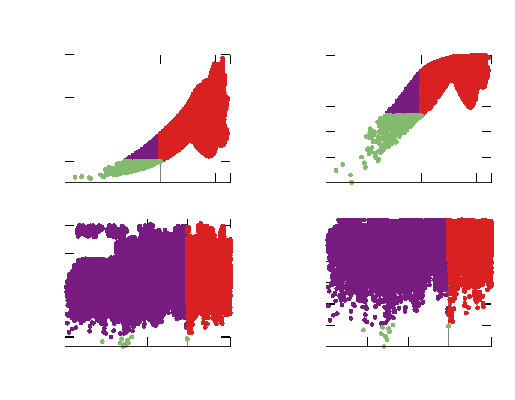
\includegraphics{./figures/h_and_h_not_fig}}%
    \gplfronttext
  \end{picture}%
\endgroup

  \vspace{0.3cm}
  \caption{\small Top: In principle there is at least one admissible pose
           estimate ($\delta \leq \delta_0$) for any choice of $k$ (Alg.
           \ref{alg:bottom_k}) in $\mathcal{H}$. However, $k$ sets threshold
           $\psi_0$ on the CAER of estimates in $\mathcal{H}$, and therefore it
           sets $\mathcal{V}$: $\mathcal{V} \cup \mathcal{X} \cup \mathcal{W} =
           \mathcal{H}$.  In case of (a) repetitions of the immediate
           environment of the sensor more than once in a given map, and (b)
           non-panoramic angular range of a sensor, as witnessed in environment
           WILLOWGARAGE (pose $\bm{p}_{i}^G$; subsection \ref{subsec:exp_b}),
           it is possible that a choice of $k$ may starve $\mathcal{V}$ of
           admissible poses. See \cite{cbglarxiv} for details on $\mathcal{V}$,
           $\mathcal{X}$, and $\mathcal{W}$
        }
        \vspace{-0.5cm}
  \label{fig:h_and_h_not_fig}
\end{figure}
